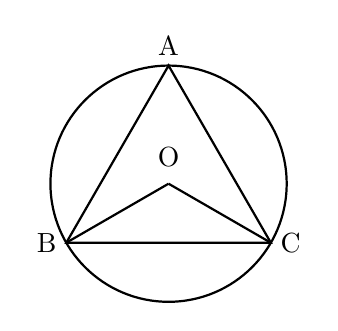
\begin{tikzpicture}[scale=1]

  % Define the center of the circle
  \coordinate (O) at (0,0);

  % Define the radius of the circle
  \def\R{1.5}

  % Draw the circle
  \draw[thick] (O) circle (\R);

  % Define the vertices of the inscribed triangle
  % A is at the top (90 degrees)
  % B and C are at the bottom left and right (approximately 210 and 330 degrees)
  \coordinate (A) at (90:\R);
  \coordinate (B) at (210:\R);
  \coordinate (C) at (330:\R);

  % Draw the triangle ABC
  \draw[thick] (A) -- (B) -- (C) -- cycle;

  % Draw the line segments from the center O to vertices B and C
  \draw[thick] (O) -- (B);
  \draw[thick] (O) -- (C);

  % Add labels for the vertices and the center exactly where they appear
  \node[above] at (A) {A};
  \node[left] at (B) {B};
  \node[right] at (C) {C};
  
  % Position the label 'O' slightly above the center intersection
  \node[above] at (0, 0.1) {O};

\end{tikzpicture}